\documentclass[12pt]{article}[margin=1in]
\usepackage{fullpage,graphicx,psfrag,amsmath,amsfonts,verbatim}
\usepackage{multicol,multirow}
\usepackage[small,bf]{caption}
\usepackage{amsthm}
\usepackage{hyperref}
\usepackage{bbm} % for the indicator function to look good
\usepackage{color}
\usepackage{mathtools}
\usepackage{fancyhdr} % for the header
\usepackage{booktabs} % for regression table display (toprule, midrule, bottomrule)
\usepackage{adjustbox} % for regression table display
\usepackage{threeparttable} % to use table notes
% \usepackage{natbib} % for bibliography
% \usepackage{minted} % for code highlighting
\usepackage{algorithm}
\usepackage{algpseudocode}
\input newcommand.tex
% \bibliographystyle{apalike}
\setlength{\parindent}{0pt} 
%\renewcommand{\thesection}{Question \arabic{section}}
% \renewcommand{\thesubsection}{\arabic{section}.\arabic{subsection}}


% Settings for page number in the footer
\pagestyle{fancy}
\fancyhf{}
\fancyfoot[C]{\thepage}
\renewcommand{\headrulewidth}{0pt}
\renewcommand{\footrulewidth}{0pt}

\title{\textbf{Solving Dynamic Oligopoly Game} \\
    \vspace{.3cm}
    \large Problem Set 2 \\
    Empirical Industrial Organization 2025 Spring}
\author{Zixuan}
\date{\today}

\begin{document}
\maketitle

\setcounter{page}{1}

\section{Tasks}
\subsection{State space}
\paragraph{Decode} See Algorithm~\ref{alg:decode}. Let's look at an example of decoding code 8 (index-0 based) to state ntuple $(2,2,1)$.
\begin{equation*}
    \begin{array}{cccccccccccc}
        0 & 1 & 1 & 1 & 2 & 2 & 2 & 2 & 2 & 2 & \ldots \\
        0 & 0 & 1 & 1 & 0 & 1 & 1 & 2 & 2 & 2 & \ldots \\
        0 & 0 & 0 & 1 & 0 & 0 & 1 & 0 & 1 & 2 & \ldots \\
    \end{array}
\end{equation*}
The trick is to make use of the following binomial coefficient matrix.
\begin{equation*}
    \begin{array}{ccccccc}
        0 & 1 &   &    &            \\
        0 & 1 & 1 &    &            \\
        0 & 1 & 2 & 1  &            \\
        0 & 1 & 3 & 3  & 1          \\
        0 & 1 & 4 & 6  & 4  & 1     \\
        0 & 1 & 5 & 10 & 10 & 5 & 1 \\
    \end{array}
\end{equation*}
We have 3 firms. For the 1st firm, we start by the value at the 3rd row. Compare the code 8 to this value, deduct the value from code, move to the bottom right by one step. Stop when the code is smaller than the value in the matrix. Then we find the state for the first position by the number of times we have moved. For the 2nd firm, we start by the alue at the 2nd row, etc.

\begin{algorithm}[!htbp]
    \caption{Decode an integer state code into a weakly descending n-tuple}
    \begin{algorithmic}[1]
        \Function{decode}{code, nfirms, binom}
        \State ntuple $\gets$ \textbf{zeros}(nfirms) \Comment{Initialize output n-tuple}

        \For{$i = 0$ to $nfirms - 1$}
        \State row $\gets$ nfirms - i - 1
        \State col $\gets$ 1
        \While{code $\geq$ binom[row, col]}
        \State code $\gets$ code - binom[row, col]
        \State row $\gets$ row + 1
        \State col $\gets$ col + 1
        \EndWhile
        \State ntuple[i] $\gets$ col - 1
        \EndFor

        \State \Return ntuple
        \EndFunction
    \end{algorithmic}
    \label{alg:decode}
\end{algorithm}

\paragraph{Encode} See Algorithm~\ref{alg:encode}. Similarly, encoding $(2,2,1)$ to code 8 is to move along the binom matrix. Summing up 1,3,1,2,1 to get 8.

\begin{algorithm}
    \caption{Encode a weakly descending n-tuple into an integer state code}
    \begin{algorithmic}[1]
        \Function{encode}{ntuple, nfirms, binom}
        \State code $\gets$ 0 \Comment{Initialize state code}

        \For{$i = 0$ to $\text{nfirms} - 1$}
        \For{$j = 0$ to $\text{ntuple}[i] - 1$}
        \State code $\gets$ code + binom[$\text{nfirms} - i - 1 + j$, $1 + j$]
        \EndFor
        \EndFor

        \State \Return code
        \EndFunction
    \end{algorithmic}
    \label{alg:encode}
\end{algorithm}

\subsection{Equilibrium computation}
\paragraph{Continuation value} Given a state ntuple $\omega$, and the position $j$ we calculate the \verb|val_up| when the firm $j$ receives a positive $\tau_j=1$ and \verb|val_up| when the firm $j$ receives $\tau_j=0$.
% \begin{algorithm}
%     \caption{Compute the continuation value of a firm in a given state}
%     \begin{algorithmic}[1]
%         \Function{calcval}
%         \Comment{I ignore the the creation of local mask here}
%         \For{$i = 0$ to rivalCombinations - 1}
%         \Comment{Compute the probability that all the rivals move to the $i$-th rivalCombinations}
%     \end{algorithmic}
% \end{algorithm}
\paragraph{Function operator} Given a set of value function $V(\omega)=\set{V_1(\omega),\ldots,V_N(\omega)}$ and policy function $x(\omega)=\set{x_1(\omega),\ldots,x_N(\omega)}$, return the new value function and policy function. This is essentially the operator which satisfies the contraction mapping theorem.

\begin{remark}
    we need to take into account two different state ntuple $\omega$ (no entry) and $\omega_e$ (with entry). Therefore, we get
    \begin{enumerate}
        \item \verb|val_up|, \verb|val_stay|
        \item \verb|val_up_e|, \verb|val_stay_e|
    \end{enumerate}
    Then the actual \verb|val_up_both| for both cases (entry or not) is taking expectation over entry. Similaryly for \verb|val_stay_both|.
\end{remark}

\begin{remark}
    The value of staying is the following, which is compared to scrap value $\phi$ to determine whether to exit.
    $$ \text{Current profit}-\text{Investment}+\beta\bra{\Pr(\tau_j=1)\text{val\_up\_both} + (1-\Pr(\tau_j=1))\text{val\_stay\_both}} $$
\end{remark}





\subsection{Simulation}
\paragraph{Code} The detail of the simulation is described in \ref{alg:simulation}. The simulation is run for 10000 periods.The initial state is $(6,0,0)$
\begin{algorithm}
    \caption{Industry Evolution Simulation}
    \begin{algorithmic}[1]
        \For{$t = 1$ to $T$}
        \Comment{Encode the current state}
        \State $\text{stateCode} \gets \text{qencode}(\text{currentState}, \text{etable}, \text{multfac})$
        \State $\text{stateHistory}[t, :] \gets \text{currentState}$
        \State $\text{firmsCountHistory}[t] \gets \sum (\text{currentState} > 0)$

        \Comment{Let potential entrant make decision (but does not enter yet!)}
        \For{$i = 1$ to $N$}
        \If{$\text{currentState}[i] = 0$}
        \State $\text{entryProb} \gets \text{isentry}[\text{stateCode}]$
        \State $\text{entry} \sim \text{Binomial}(1, \text{entryProb})$
        \If{$\text{entry}$}

        \State $\text{entryIndex} \gets i$
        \Comment{Get the position of the vacancy where one entrant enters.}
        \EndIf

        \State \textbf{break}
        \Comment{Only one entrant can enter.}
        \EndIf
        \EndFor

        \Comment{Let firms make exit decision and exit.}\\
        \Comment{The currentState is not in descending order}\\
        \Comment{This is necessary when we retrieve value and policy from newvalue and newx}
        \State $\text{sortedIndex} \gets \text{argsort} (\text{currentState})[::-1]$
        \For{$j = 1$ to $N$}
        \If{$\text{newvalue}[\text{stateCode}, :][\text{sortedIndex}][j] < \phi$}
        \State $\text{currentState}[j] \gets 0$
        \State $\text{currentState}[\text{currentState} \leq \text{currentState}[j]] \gets 0$
        \EndIf
        \EndFor

        \Comment{Investment decision}
        \State $\text{investmentPolicyolicy} \gets (\text{currentState} > 0) * (\text{newx}[\text{stateCode}, :][\text{sortedIndex}])$
        \State $\text{investmentHistory}[t, :] \gets \text{investmentPolicyolicy}$
        \Comment{Let entrant enter!}
        \If{$\text{entry}$}
        \State $\text{currentState}[\text{entryIndex}] \gets \text{entryLevel}$
        \EndIf

        \Comment{Simulate individual shocks}
        \State $\Pr(\tau_j = 1) \gets \frac{a \cdot \text{investmentPolicyolicy}}{1 + a \cdot \text{investmentPolicyolicy}}$
        \State $\tau_j \sim \text{Binomial}(1, \Pr(\tau_j = 1))$

        \Comment{Update industry state}
        \State $\text{currentState} \gets \max(\min(\text{currentState} + \text{individual\_shocks} - \nu[t], kmax), 0)$
        \EndFor
    \end{algorithmic}
    \label{alg:simulation}
\end{algorithm}

\paragraph{Results} The statistics of the simulation results are shown in Table \ref{tab:simulation_results}. I also plot the trajectory of \textbf{firms count} and \textbf{average investment per period}. Since the number of time period is too large, for visualisation purpose I restrict myself to the first and last 100 periods. (It seems that investment is converging to zero...)

\begin{table}[!htbp]
    \centering
    \begin{tabular}{lcc}
        \toprule
                       & Firms Count & Average Investment \\
        \midrule
        Baseline       & 2.2799      & 0.1904             \\
        Low Entry Cost & 2.6627      & 0.1692             \\
        \bottomrule
    \end{tabular}
    \caption{Simulation Results}
    \label{tab:simulation_results}
\end{table}

\newpage
\begin{figure}[!htbp]
    \centering
    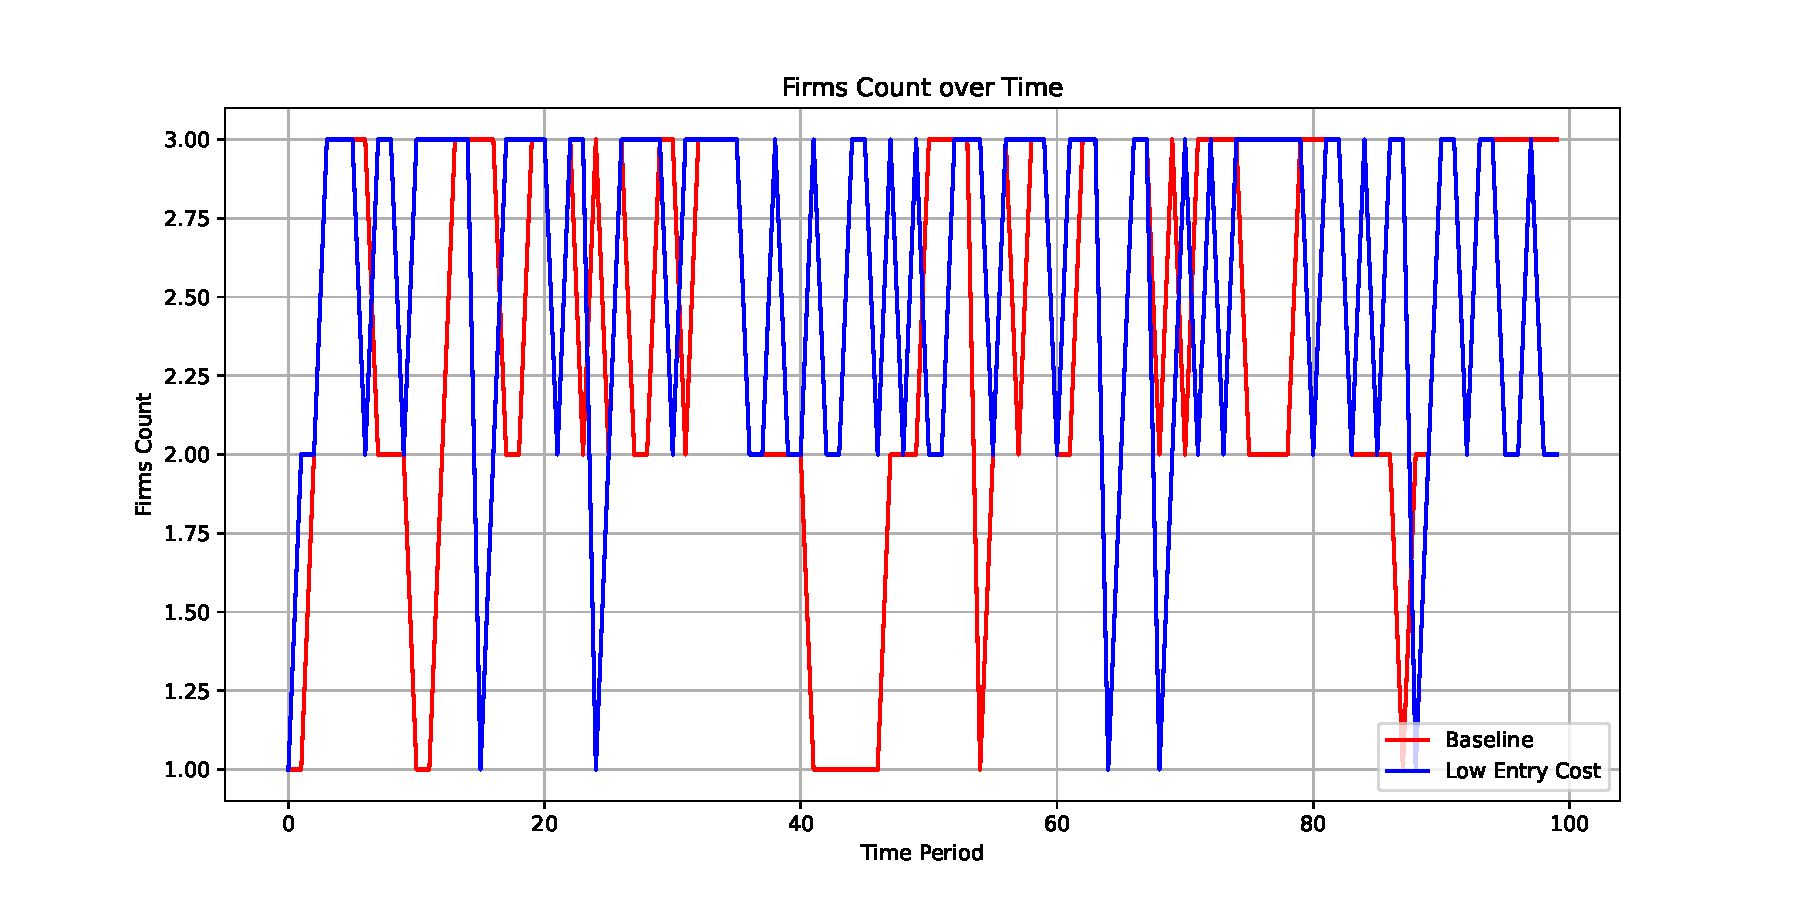
\includegraphics[width=0.8\textwidth]{../Figures/Firms_count_start.pdf}
    \caption{Firms Count Trajectory (First 100 periods)}
\end{figure}
\begin{figure}[!htbp]
    \centering
    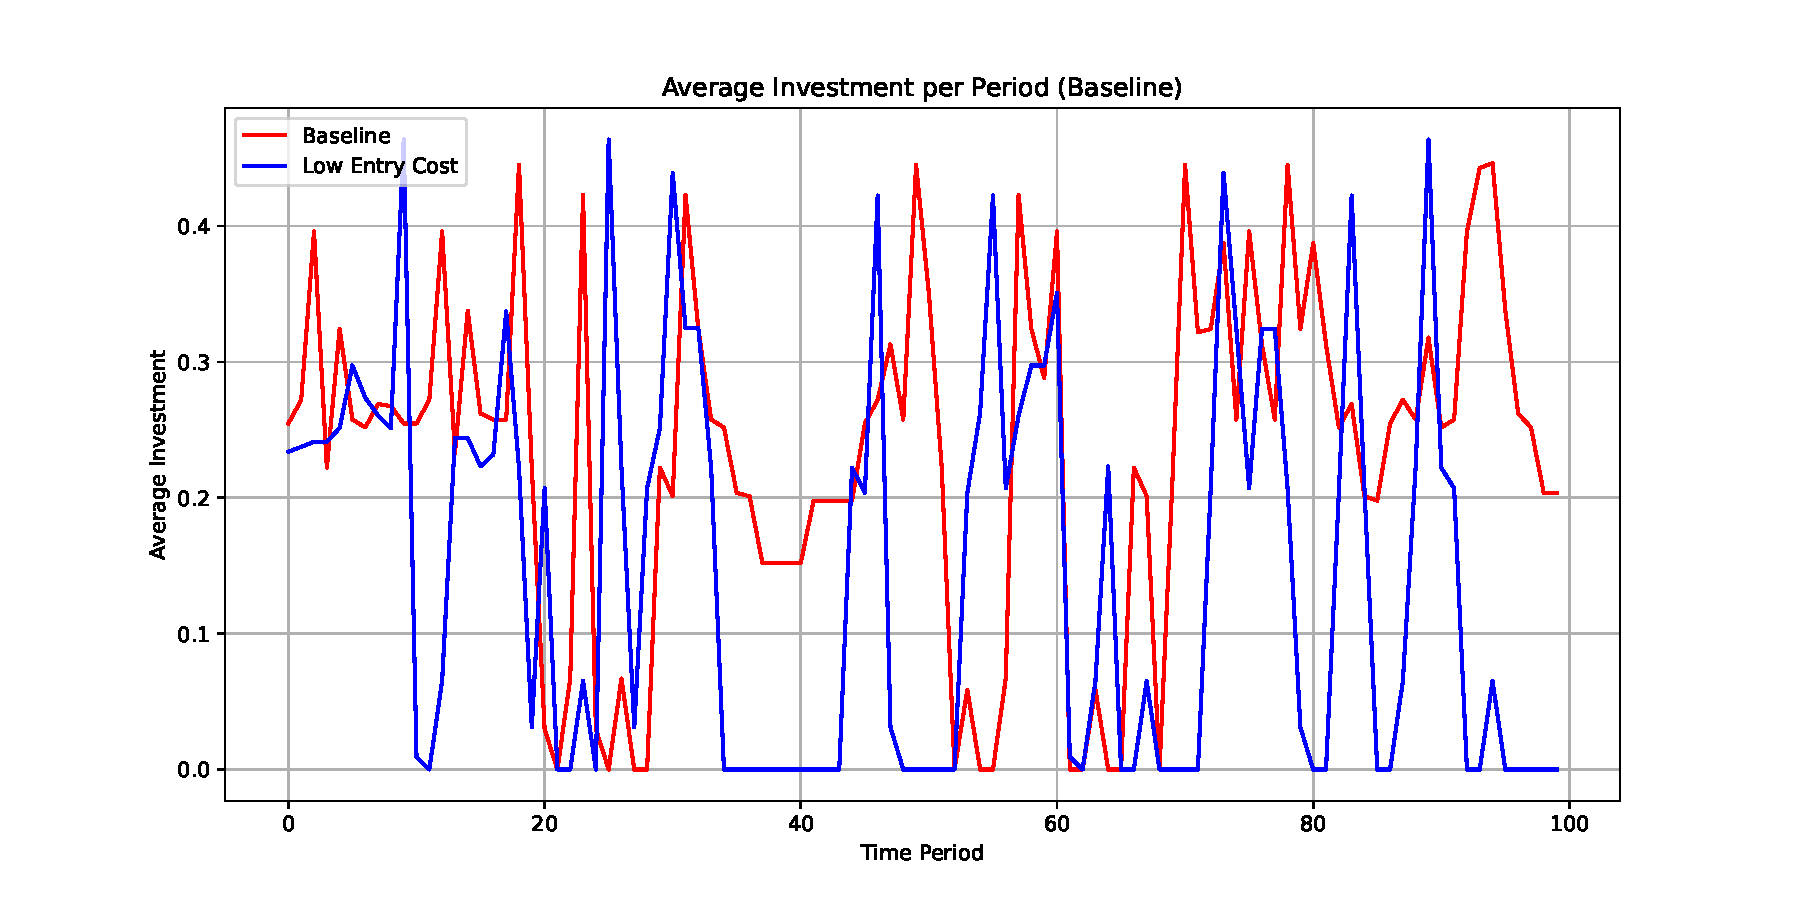
\includegraphics[width=0.8\textwidth]{../Figures/Average_investment_trajectory_start.pdf}
    \caption{Average Investment Trajectory (First 100 periods)}
\end{figure}

\newpage
\begin{figure}[!htbp]
    \centering
    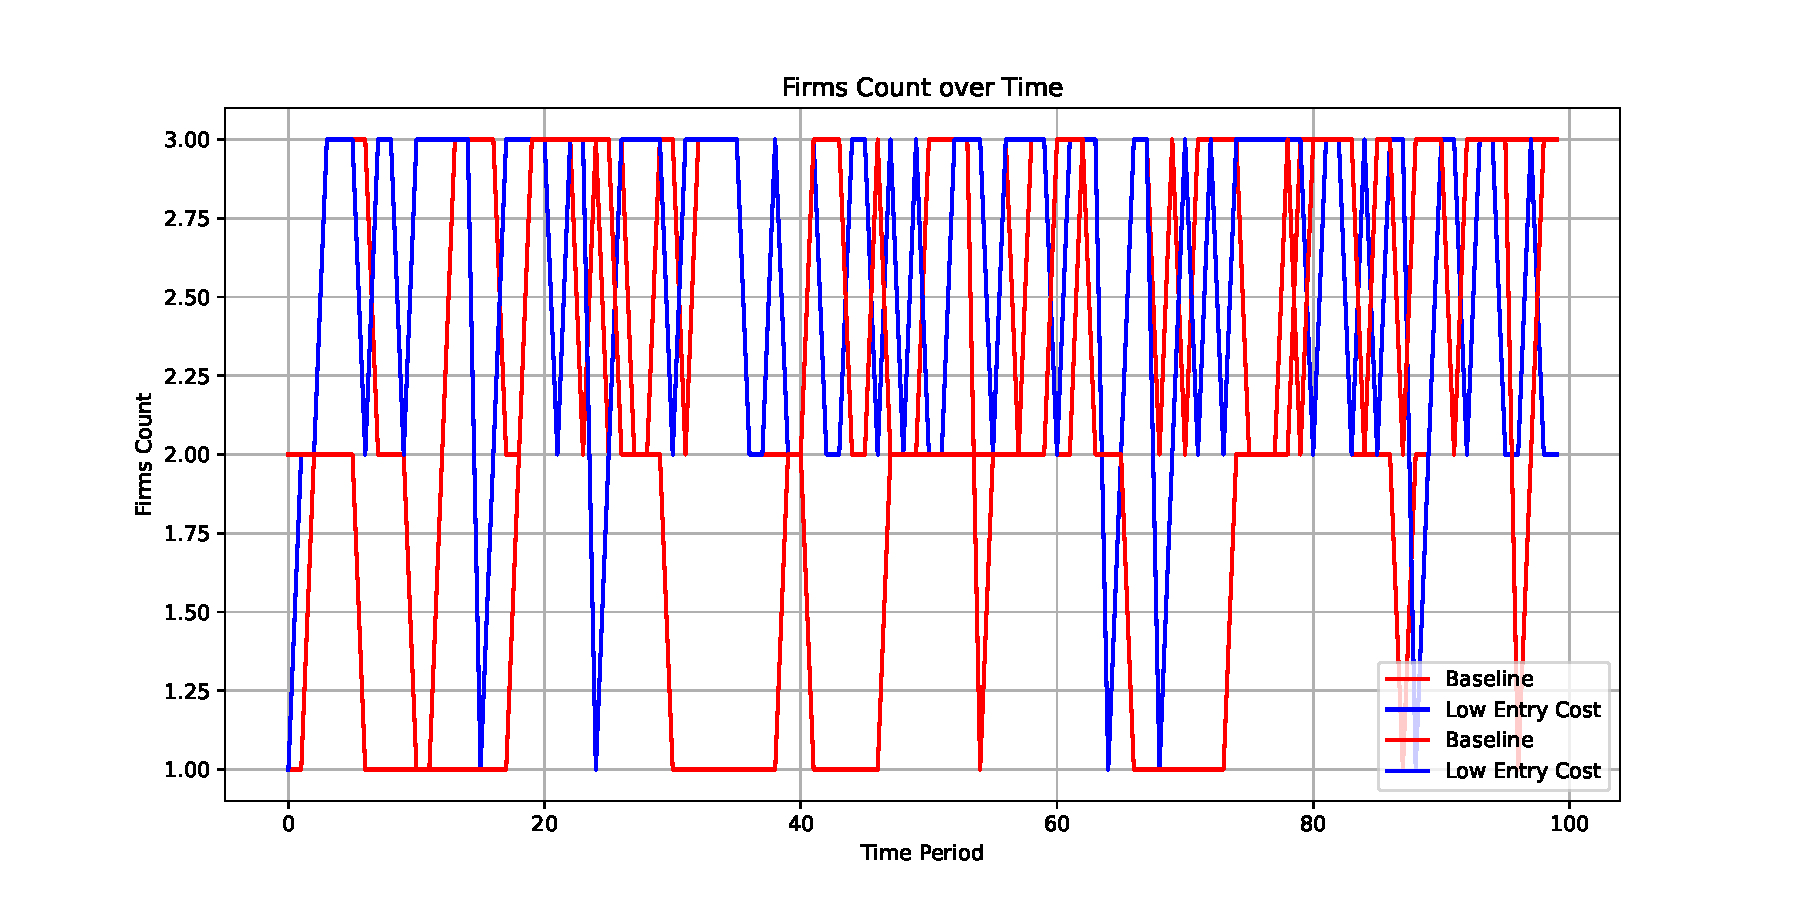
\includegraphics[width=0.8\textwidth]{../Figures/Firms_count_end.pdf}
    \caption{Firms Count Trajectory (Last 100 periods)}
\end{figure}
\begin{figure}[!htbp]
    \centering
    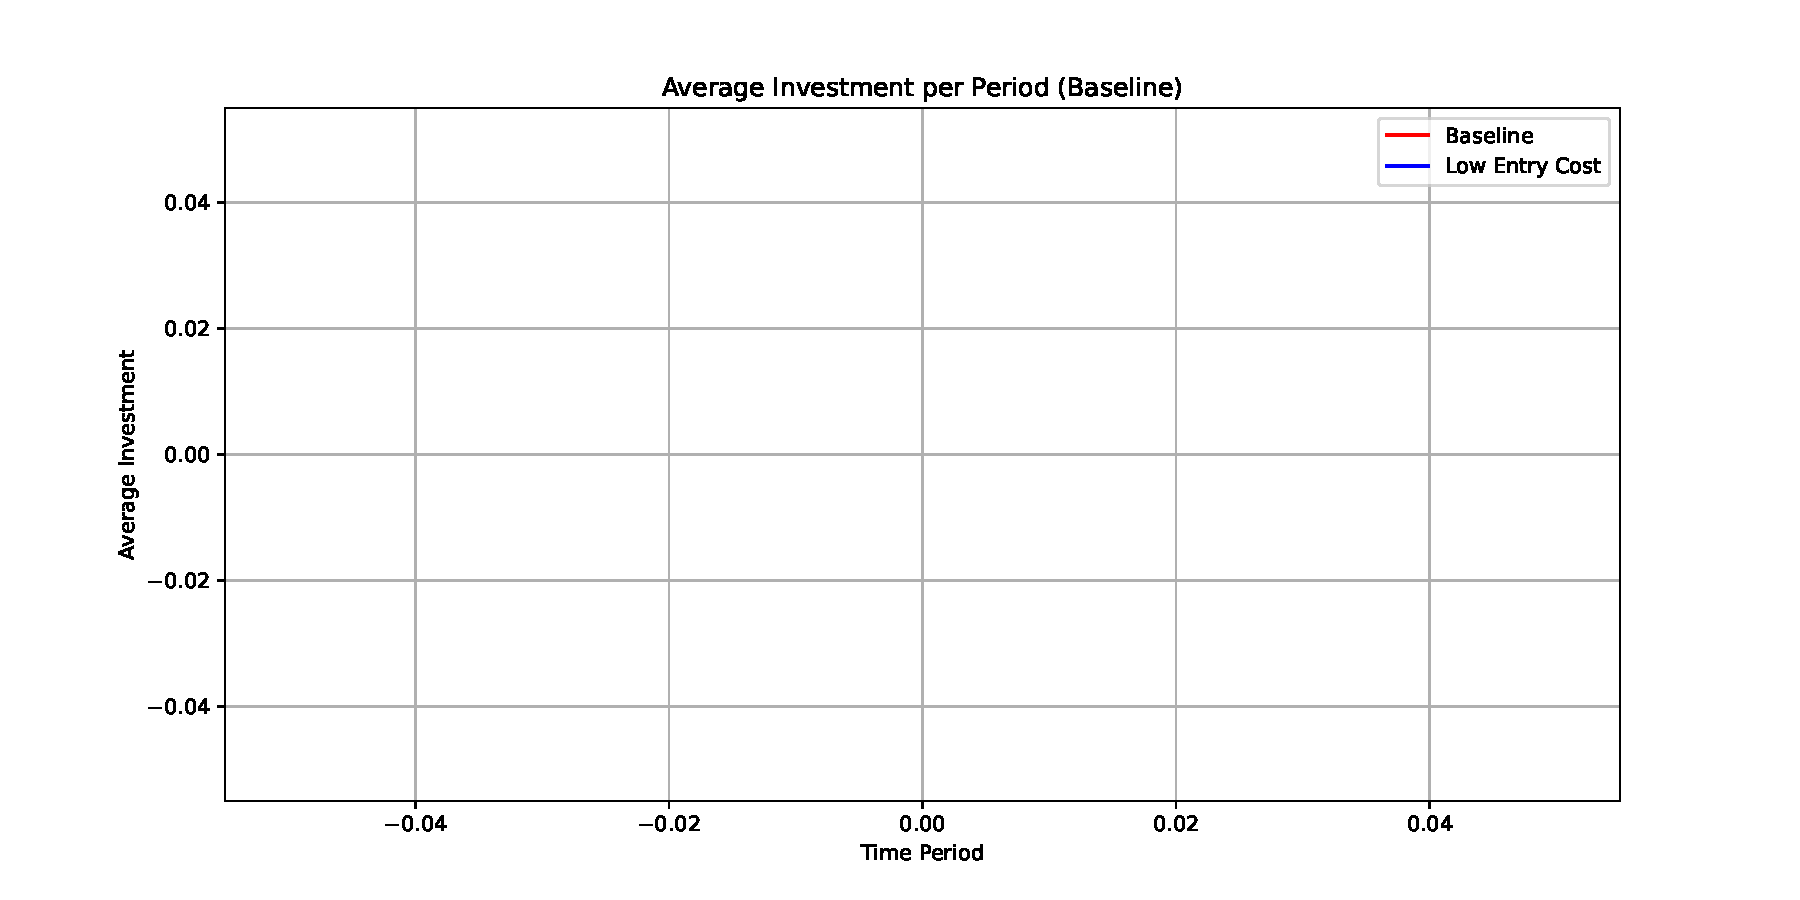
\includegraphics[width=0.8\textwidth]{../Figures/Average_investment_trajectory_end.pdf}
    \caption{Average Investment Trajectory (Last 100 periods)}
\end{figure}


% \newpage
% \bibliography{../References/ref.bib}


\end{document}